\section{Overview}\label{sec:overview}

% \begin{figure}
%   \centering
%   \begin{subfigure}[t]{0.4\textwidth}
%     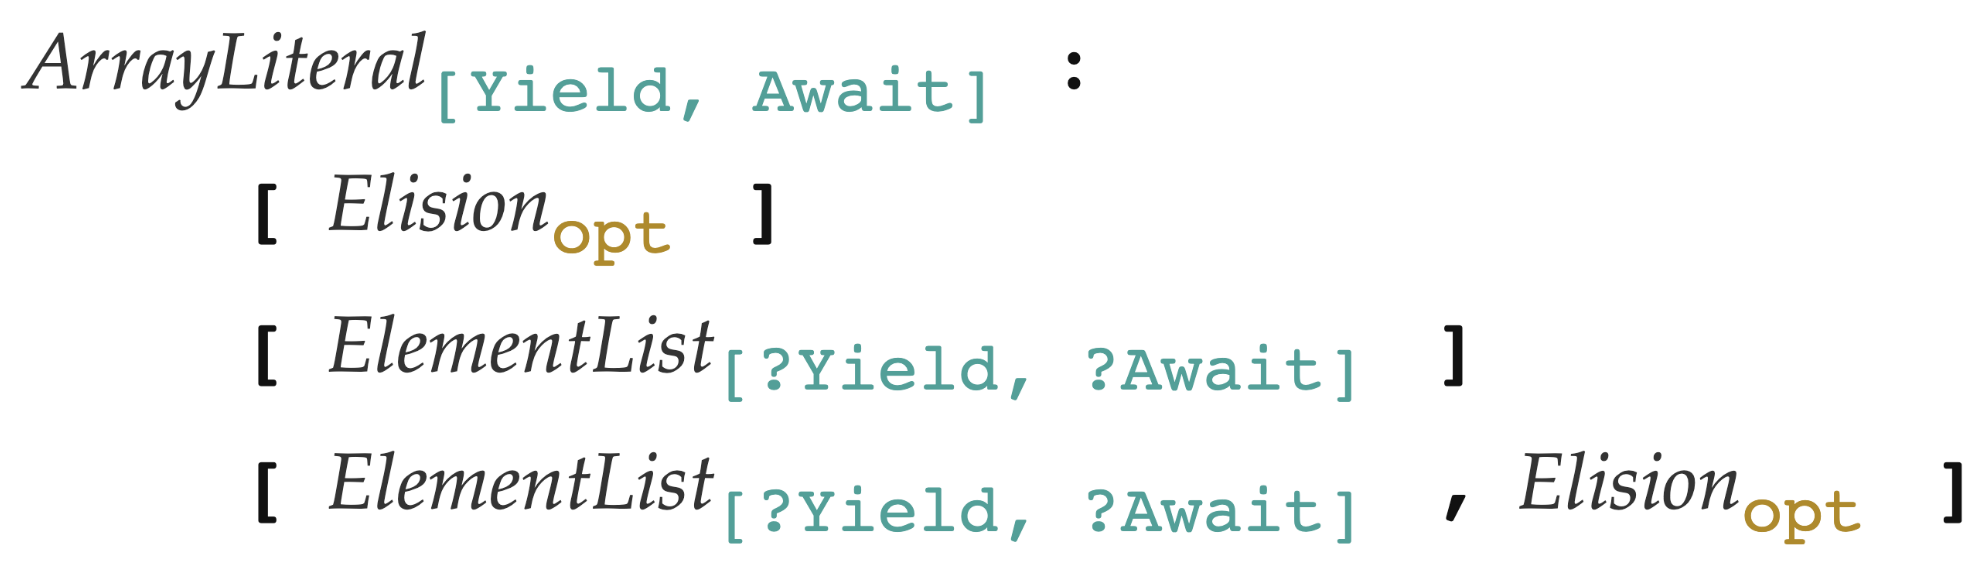
\includegraphics[width=\textwidth]{img/arrayliteral-syntax}
%     \caption{\textit{ArrayLiteral} production in ES10}
%     \label{fig:array-literal-es}
%   \end{subfigure}
%   \begin{subfigure}[t]{0.48\textwidth}
%     \begin{lstlisting}[style=myScalastyle]
% val ArrayLiteral: List[Boolean] => LAParser[T] = memo {
%   case List(Yield, Await) =>
%   "[" ~ opt(Elision) ~ "]"             ^^ ArrayLiteral0 |
%   "[" ~ ElementList(Yield,Await) ~ "]" ^^ ArrayLiteral1 |
%   "[" ~ ElementList(Yield,Await) ~ ","
%       ~ opt(Elision)~ "]"              ^^ ArrayLiteral2
% }
%     \end{lstlisting}
%     \vspace*{-1em}
%     \caption{Generated parser for the \textit{ArrayLiteral} production}
%     \label{fig:array-literal-parser}
%   \end{subfigure}
%   \vspace*{-1em}
%   \caption{\textit{ArrayLiteral} production in ES10 and its parser}
%   \label{fig:array-literal}
% \end{figure}

In this section, we demonstrate overall structure of $\tool$ depicted in
Figure~\ref{}

\subsection{Motivation}
\subsection{Overall Structure}
